\documentclass[a4paper]{article}

\usepackage[utf8]{inputenc}
\usepackage[pdftex]{graphicx}
\usepackage{amsmath,tabu,url}
\usepackage{listings}
\usepackage{array}
\usepackage{pgf}
\usepackage{tikz}
\usetikzlibrary{positioning}
\usetikzlibrary{arrows}

\setlength{\parskip}{.7ex}
\newcommand{\HRule}{\rule{\linewidth}{0.5mm}}
\renewcommand{\mod}{\,\%\,}
\renewcommand{\labelitemi}{$\circ$}
\let\olditemize\itemize
\renewcommand{\itemize}{
    \olditemize
    \setlength{\itemsep}{3pt}
    \setlength{\parskip}{0pt}
}
\lstnewenvironment{code}[1][]%
{
   \noindent
   \minipage{\linewidth} 
   \vspace{0.5\baselineskip}
   \lstset{basicstyle=\ttfamily\footnotesize,frame=single,#1}}
{\endminipage}
\title{Minimum Spanning Tree}
\begin{document}

\begin{titlepage}
\begin{center}

% Upper part of the page. The '~' is needed because \\
% only works if a paragraph has started.

\includegraphics[width=0.3\textwidth]{./img/beoi-logo}~\\[1cm]

\textsc{\LARGE Belgian Olympiad in Informatics}\\[1.5cm]

\textsc{\Large Easter Training --- Day 3}\\[0.5cm]

% Title
\HRule \\[0.4cm]
{ \huge \bfseries Competitive programming algorithms and \\ Contest Strategies \\[0.4cm] }

\HRule \\[1.5cm]

% Author and supervisor
\begin{center} \large
\emph{Trainer:}\\
Floris \textsc{Kint}
\end{center}

\vfill

% Bottom of the page
{\large \today}

\end{center}
\end{titlepage}


\tableofcontents

\section{Minimum spanning tree}
Finding a minimum spanning tree is a problem that frequently occurs in programming contests.
\subsection{Introduction}
\subsubsection{Formal definition}
Given a graph $G$ with edges $E$ and vertices $V$.
A spanning tree $T$ of $G$ is a tree that connects all vertices in $V$. The cost of the spanning tree is the sum of its edge weights.
A minimum spanning tree (MST) of $G$ is a spanning tree of $G$ that has a minimal cost. That is, no spanning tree of $G$ exists with a cost lower than the cost of $T$.

\subsubsection{Intuition}
Consider the following situation:
Given a set of cities and no roads. You want all cities to be reachable from any other city. You don't care about the traveling time, but you do care about the total price of constructing those roads. The price of constructing a road is proportional to the distance between the cities it connects. Determine which roads you need to construct.

The problem above is a typical minimum spanning tree problem. The original graph G has edges between every pair of cities (the roads). The weights of the edges are the costs of the roads they represent. Your task is to select a subset of edges (roads) such that all cities are connected (reachable from every other city). The subset you're trying to find should have a minimal total edge weight (road cost).

\subsubsection{Properties}
\textit{We consider graphs with only positive edge weights.}

A minimum spanning tree of a graph $G$ with $n$ vertices, consists of $n-1$ edges (like any tree).

\subsection{Prim's algorithm}
A first algorithm that can find a minimum spanning tree of a graph, is called Prim's algorithm. The algorithm is very similar to Dijkstra's algorithm.
\subsubsection{The algorithm}
The algorithm first takes an arbitrary vertex of the original graph as the current tree. It then repeatedly selects the closest vertex of the graph to the tree. An easy way to implement this is by using a priority queue. The code can be found in Listing~\ref{code-prim}.

\lstinputlisting[label=code-prim,caption=Prim's algorithm, language=C++,firstline=21, lastline=40, tabsize=2, breaklines=true, numbers=left, float]{src/prim.cpp}
\subsubsection{Complexity}
The algorithm iterates over all neighbours of every node in the graph. This is equivalent to iterating over all edges twice. In each of those iterations, it adds one node to the priority queue. The priority queue can contain $O(V^2)$ nodes, so this operation takes $O(\log{V^2}) = O(\log{V})$ time. Thus, the algorithm runs in $O(E \log{V})$.
\subsection{Kruskal's algorithm}
A second algorithm that can construct a minimum spanning tree, was written by Joseph Kruskal.
\subsubsection{The algorithm}
Kruskal's algorithm builds a forest (set of trees) which it merges by selecting the shortest available edges.

In the beginning, every node is a separate tree. Next, the algorithm keeps finding the edge with the lowest weight which has not been considered yet. If this edge connects two unlinked trees, the edge is added to the forest. If not, it is discarded.
The code can be found in Listing~\ref{code-kruskal}.
\lstinputlisting[label=code-kruskal,caption=Kruskal's algorithm, language=C++,firstline=49, lastline=64, tabsize=2, breaklines=true, numbers=left, float]{src/kruskal.cpp}
\subsubsection{Union-find}
Merging two trees and checking whether two nodes are in the same three can easily be done using a Union-Find data structure.
The code can be found in Listing~\ref{code-kruskal-union-find}.
\lstinputlisting[label=code-kruskal-union-find,caption=Union find, language=C++,firstline=27, lastline=46, tabsize=2, breaklines=true, numbers=left, float]{src/kruskal.cpp}

\subsubsection{Complexity}
The algorithm first sorts all edges ($O(E\log{E})$).
The algorithm iterates over all edges. For each of them, it checks whether the two endpoints are in the same tree and possibly merges the two trees. The tree a node belongs to can only change $n-1$ times during the execution of the algorithm. The function \textit{find\_parent} runs in $O(1)$ except for when the structure of its tree has changed, in which case the function cannot take more than $O(\log{V})$. 

Overall this means that the algorithm runs in $O(E\log{E}) + O(E \log{V}) = O(E \log{V})$.
\subsection{Exercises}

\begin{enumerate}
\item http://uva.onlinejudge.org/external/5/544.html
\item http://uva.onlinejudge.org/external/117/p11710.pdf (Try to use both algorithms)
\item http://uva.onlinejudge.org/external/101/p10147.pdf
\end{enumerate}
\section{Topological sorting}

\subsection{Introduction}

\subsubsection{An introductory problem}
You have a number $n$ of tasks to do, and each task have some dependencies over some other tasks that has to be done before.

If I give you these tasks and the list of their dependencies, can you give me the order in which I have to do the tasks?

\begin{center}
  \begin{tabular}{|l|l|}
  \hline
  \textbf{Task} & \textbf{Dependencies}\\
  \hline
  0 & 1,2,3\\
  1 & 2,4\\
  2 & 4\\
  3 & 1,2\\
  4 & -\\
  5 & 1\\
  \hline
  \end{tabular}
\end{center}

This can be viewed as a directed\footnote{In this problem, it is also acyclic. Why?} graph:

\begin{center}
  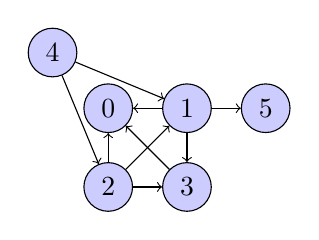
\begin{tikzpicture}[->,nodes={draw, fill=blue!20, circle},row sep=0.3cm,column sep=0.5cm]
    \node (4) {4};
    \node (0) [below right of=4] {0};

    \node (1) [right of=0] {1};
    \node (2) [below of=0] {2};
    \node (3) [right of=2] {3};
    \node (5) [right of=1] {5};

    \draw (1) -> (0);
    \draw (2) -> (0);
    \draw (3) -> (0);
    \draw (2) -> (1);
    \draw (4) -> (1);
    \draw (4) -> (2);
    \draw (1) -> (3);
    \draw (2) -> (3);
    \draw (1) -> (5);
  \end{tikzpicture}
\end{center}

The solution can be derived from a reordering of the vertices:
\begin{center}
  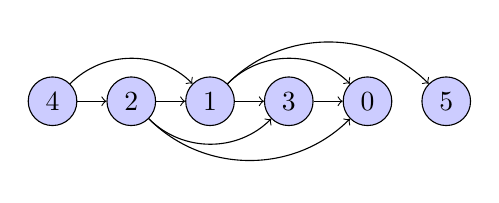
\begin{tikzpicture}[->,nodes={draw, fill=blue!20, circle},row sep=0.3cm,column sep=0.5cm]
    \node (4) {4};
    \node (2) [right of=4] {2};
    \node (1) [right of=2] {1};
    \node (3) [right of=1] {3};
    \node (0) [right of=3] {0};
    \node (5) [right of=0] {5};

    \draw [->] (1) to [bend left=45] (0);
    \draw [->] (2) to [bend right=45] (0);
    \draw (3) -> (0);
    \draw (2) -> (1);
    \draw [->] (4) to [bend left=45] (1);
    \draw (4) -> (2);
    \draw (1) -> (3);
    \draw [->] (2) to [bend right=45] (3);
    \draw [->] (1) to [bend left=45] (5);
  \end{tikzpicture}
\end{center}
\subsubsection{Definition}
A \textbf{topological sort} (sometimes called \textit{toposort}) is an ordering of the vertices of a directed graph, such that, if there is an edge linking vertex $u$ to vertex $v$, we have that $u$ comes before $v$ in the ordering.

\subsubsection{Properties}
\begin{itemize}
\item A topological sort exists for a given graph if and only if there is no directed cycles $==$ if it is a Directed Acyclic Graph (DAG)
\item Every DAG has a valid topological sort;
\item A given DAG may have more than one toposort (for example, our earlier examples accepts three toposorts);
\item If there is a path linking vertices $u$ and $v$, you have that $u$ comes before $v$ in the toposort.
\end{itemize}


\subsection{Algorithm}
The topological sort is in fact the inverse order followed by the DFS \textbf{when "closing" the vertices}.

\begin{lstlisting}[label=code-dfs,caption=DFS algorithm, language=Java, tabsize=2, breaklines=true, numbers=left]
int UNVISITED = 0, OPEN = 1, CLOSED = 2;

void dfsVisit(LinkedList<Integer>[] adj_list, int node, int[] labels)
{
	labels[node] = OPEN;
	for(int new_node : adj_list[node])
		if(labels[new_node] == UNVISITED)
			dfsVisit(adj_list, new_node, labels);
	labels[node] = CLOSED;
}

void dfs(LinkedList<Integer>[] adj_list)
{
	int[] labels = new int[adj_list.length];
	Arrays.fill(labels, UNVISITED);
	for(int node = 0; node < adj_list.length; node++)
		if(labels[node] == UNVISITED)
			dfsVisit(adj_list, node, labels);
}
\end{lstlisting}

When a node $u$ is marked as \texttt{CLOSED}, you have that all nodes to which there is a path from $u$ have already been closed; that means that they lies \textbf{after} $u$ in the toposort.

When then only have to remember the order in which the nodes are closed, and reverse it. We do that using a stack:

\begin{lstlisting}[label=code-toposort,caption=Toposort algorithm, language=Java, tabsize=2, breaklines=true, numbers=left]
int UNVISITED = 0, OPEN = 1, CLOSED = 2;

void dfsVisit(LinkedList<Integer>[] adj_list, int node, int[] labels, Stack<Integer> stack)
{
	labels[node] = OPEN;
	for(int new_node : adj_list[node])
		if(labels[new_node] == UNVISITED)
			dfsVisit(adj_list, new_node, labels, stack);
	labels[node] = CLOSED;
    stack.push(node);
}

Stack<Integer> toposort(LinkedList<Integer>[] adj_list)
{
	int[] labels = new int[adj_list.length];
    Stack<Integer> stack = new Stack<Integer>();
    
	Arrays.fill(labels, UNVISITED);
	for(int node = 0; node < adj_list.length; node++)
		if(labels[node] == UNVISITED)
			dfsVisit(adj_list, node, labels, stack);
    return stack;
}
\end{lstlisting}

\subsection{Exercises}
\begin{enumerate}
\item Do the problem 200 from UVA: \url{http://uva.onlinejudge.org/index.php?option=com_onlinejudge&Itemid=8&page=show_problem&category=24&problem=136}
\item Bonus: do the problem 872 from UVA: \url{http://uva.onlinejudge.org/external/8/872.html}
\end{enumerate}
\section{Eulerian paths and tours}
\subsection{The seven bridges of Königsberg}
Königsberg, in Prussia\footnote{now called Kaliningrad, Russia}, was traversed by a river, creating two small island. They were seven gates that allowed to go from one part of Königsberg to the other.

As the bridges of Königsberg were probably very beautiful, citizens wanted to create a path that crossed each bridge once. An unknown guy, named Leonard Euler, decided to tackle this problem. The figure below\footnote{Taken from Wikipedia...} shows the bridges of Königsberg.

\begin{center}
	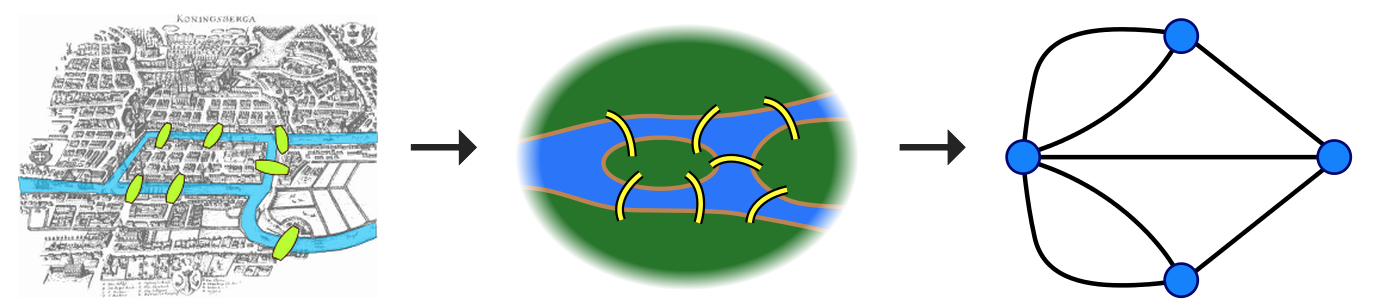
\includegraphics[width=\textwidth]{./img/konisberg.png}
\end{center}

Euler worked a bit on the problem, and saw that, in fact, he simply could invent graph theory to prove that there was no such path.

\subsection{Definitions}
\begin{itemize}
\item The degree of a node $v$, noted $\#v$, is the number of edges that are connected to this node. Edges that are loops (that connect a node to itself) count double.
\item An Eulerian path\footnote{Also called Eulerian trail} in a graph is a path that cross each edge of the graph once.
\item An Eulerian tour\footnote{Also called Eulerian cycle} is an Eulerian path that is also a cycle.
\end{itemize}

Euler then searched an Eulerian\footnote{yep, he was a bit self-centered} path in Königsberg.

\subsection{Properties}
After some hours thinking on the problem, he wrote some theorems:

\begin{itemize}
\item The sum of the degree for all nodes equals to two times the number of edges (all edges are linked to two nodes).
\item A graph contains an Eulerian tour if and only if all nodes have an even degree. \footnote{Here is the intuition for the demo: when you enter in a node, you "consume" one degree related to the inbound edge, and when you exit a node, you "consume" another degree related to the outbound edge. Thus, you consume two "part of degree" each time you go throughout a node.}
\item A graph contains an Eulerian path if and only if there is at most two nodes with an odd degree. 
\end{itemize}

\subsection{Hierholzer's Algorithm}
The Hierholzer's algorithm is used to find Eulerian tours\footnote{It can be easily expanded to find Eulerian paths: you just have to add an edge between the two nodes that have an odd degree, run the algorithm to produce the Eulerian tour, then delete the added edge!} in graph.

It is very simple: you simply start from a random vertex $u$, then follow one edge to another vertex (mark the edge as used), etc, until you reach again $u$. You have then formed a cycle that "uses" some of the edges. If there are still edges available on $u$, repeat the operation, and then merge the cycles, etc. If there are no longer unused edges starting from $u$, then go to the next vertex in the cycle, and repeat everything.

\begin{lstlisting}[label=code-eulerian,caption=Hierholzer's Algorithm, language=Java, tabsize=2, breaklines=true, numbers=left]
LinkedList<Integer> eulerianCycle(LinkedList<Integer>[] adj_list)
{
	//For simplicity, we assume that the graph is connected...
		
	LinkedList<Integer> cycle = new LinkedList<Integer>();
	cycle.add(0); //add an initial node
		
	//Iterate throught the cycle
	ListIterator<Integer> listIterator = cycle.listIterator();
    while (listIterator.hasNext())
    {
    	int new_start = listIterator.next();
    	//If we can begin a new cycle...
    	if(adj_list[new_start].size() != 0)
    	{
    		int current = new_start;
    		int size_added = 0;
    		do
    		{
    			int next_node = adj_list[current].poll();

				//delete the edge in the other direction
				//this is slow and can be improved using a separate Set
				adj_list[next_node].remove(new Integer(current));

				current = next_node;
				listIterator.add(current);
				size_added++;
			} while(current != new_start);

			//go back to the initial node, to verify there is no other edges
			for (int i = 0; i < size_added; i++)
				listIterator.previous();
		}
	}
	return cycle;
}
\end{lstlisting}

This algorithm runs in linear time, depending only of the number of vertices and edges: $O(|V|+|E|)$.

\subsection{Exercises}
\begin{enumerate}
\item Do the problem 10054 from UVA: \url{http://uva.onlinejudge.org/external/100/p10054.pdf}.
\textbf{Warning}: there is lot of input/output, so, in Java, use BufferedReader and BufferedWriter!
\item Bonus: do the problem 10596 from UVA: \url{http://uva.onlinejudge.org/index.php?option=com_onlinejudge&Itemid=8&category=24&page=show_problem&problem=1537}
\end{enumerate}
\section{Strongly Connected Components}
\subsection{Introduction}
Strongly Connected Components (SCC) are an extension of the concept of connexity for directed graphs.

A strongly connected component is a sub-graph in which there is a (directed) path from each vertex of the component to each vertex of the component.

An example is given in the graph below. There are three strongly connected components.
\begin{center}
  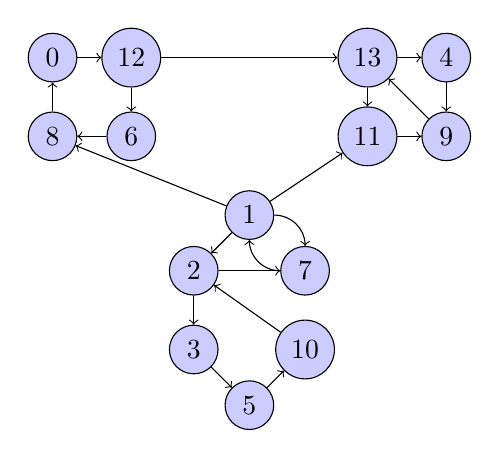
\begin{tikzpicture}[->,nodes={draw, fill=blue!20, circle},row sep=0.3cm,column sep=1cm]
    \node (a0) {0};
    \node (a1) [right of=a0] {12};
	\node (a2) [below of=a1] {6};
    \node (a3) [left of=a2] {8};
    
    \node (b0) [right of=a1,xshift=2cm] {13};
    \node (b1) [right of=b0] {4};
    \node (b2) [below of=b1] {9};
    \node (b3) [left of=b2] {11};
    
    \node (c0) [below of=a3,yshift=-0cm,xshift=2.5cm] {1};
    \node (c1) [below right of=c0] {7};
    \node (c2) [below left of=c0] {2};
    \node (c3) [below of=c1] {10};
    \node (c4) [below of=c2] {3};
    \node (c5) [below right of=c4] {5};
    
    \draw (a0) -> (a1);
    \draw (a1) -> (a2);
    \draw (a2) -> (a3);
    \draw (a3) -> (a0);
    
    \draw (b0) -> (b1);
    \draw (b0) -> (b3);
    \draw (b1) -> (b2);
    \draw (b3) -> (b2);
    \draw (b2) -> (b0);
    
    \draw (c0) -> (c2);
    \draw [->] (c1) to [bend left=45] (c0);
    \draw [->] (c0) to [bend left=45] (c1);
    \draw (c2) -> (c4);
    \draw (c4) -> (c5);
    \draw (c5) -> (c3);
    \draw (c3) -> (c2);
    \draw (c2) -> (c1);
    
    \draw (c0) -> (a3);
    \draw (c0) -> (b3);
    \draw (a1) -> (b0);
  \end{tikzpicture}
\end{center}

\subsection{Properties}
\begin{itemize}
\item Inside a SCC, you are sure that there is a path from everywhere to everywhere;
\item If you contract each SCCs to a single vertex, the resulting graph is a DAG;
\item A transposed graph has the same SCCs as the original one.
\end{itemize}

\subsection{Algorithm}
\subsubsection{Using topological sort}
After having performed the topological sort of the graph, you can use DFS \textbf{using topological order on the transposed graph} to find the SCCs.

The intuition is rather simple: the toposort algorithm on the complete graph will more or less give you the toposort of the DAG of the SCCs; transposing the graph will then allow you to only access the current SCC; each DFS call on a node will give you a new SCC.

\begin{lstlisting}[label=code-scc1,caption=Toposort+DFS, language=Java, tabsize=2, breaklines=true, numbers=left]
void dfsVisit(LinkedList<Integer>[] adj_list, int node, int start_node, int[] labels, Stack<Integer> stack)
{
	labels[node] = OPEN;
	for(int new_node : adj_list[node])
		if(labels[new_node] == UNVISITED)
			dfsVisit(adj_list, new_node, start_node, labels, stack);
	//small change to original DFS: instead of CLOSED, mark nodes as the "start node"
	labels[node] = start_node;
	stack.push(node);
}

LinkedList<Integer>[] transpose(LinkedList<Integer>[] a)
{
	LinkedList<Integer>[] b = new LinkedList[a.length];
	for (int i = 0; i < b.length; i++)
		b[i] = new LinkedList<Integer>();
	for (int i = 0; i < a.length; i++)
		for (int j: a[i])
			b[j].add(i);
	return b;
}

int[] scc(LinkedList<Integer>[] adj_list)
{
	//first, run toposort
	int[] labels = new int[adj_list.length];
	Stack<Integer> stack = new Stack<Integer>();

	Arrays.fill(labels, UNVISITED);
	for(int node = 0; node < adj_list.length; node++)
		if(labels[node] == UNVISITED)
			dfsVisit(adj_list, node, node, labels, stack);

	//run dfsVisit following the toposort order
	labels = new int[adj_list.length];
	LinkedList<Integer>[] adj_list_transposed = transpose(adj_list);
	Arrays.fill(labels, UNVISITED);
	while(!stack.isEmpty())
	{
		int node = stack.pop();
		if(labels[node] == UNVISITED)
			dfsVisit(adj_list_transposed, node, node, labels, stack);
	}

	//Labels now contains the ids of the SCCs.
	return labels;
}
\end{lstlisting}

\subsection{Tarjan's algorithm}
Tarjan's algorithm use a completely different approach, and uses only a single DFS.
It is however less simple to explain, to understand and to use in contests.

\begin{lstlisting}[label=code-scc2,caption=Toposort+DFS, language=Java, tabsize=2, breaklines=true, numbers=left]
int UNVISITED = -1;
int[] dfs_low;
int[] dfs_num;
boolean[] is_in_stack;
Stack<Integer> stack;
int num;
LinkedList< LinkedList<Integer> > sccs;
	
void tarjanVisit(LinkedList<Integer>[] adj_list, int node)
{
	dfs_low[node] = dfs_num[node] = num;
	num++;
	stack.push(node);
	is_in_stack[node] = true;

	for(int s: adj_list[node])
	{
		if(dfs_num[s] == UNVISITED)
		{
			tarjanVisit(adj_list, s);
			dfs_low[node] = Math.min(dfs_low[node], dfs_low[s]);
		}
		else if(is_in_stack[s])
		{
			dfs_low[node] = Math.min(dfs_low[node], dfs_num[s]);
		}
	}
		
	if(dfs_low[node] == dfs_num[node])
	{
		LinkedList<Integer> scc = new LinkedList<Integer>();
		int t;
		do
		{
			t = stack.pop();
			is_in_stack[t] = false;
			scc.add(t);
		} while(t != node);
		sccs.add(scc);
	}
}
	
LinkedList< LinkedList<Integer> > tarjan(LinkedList<Integer>[] adj_list)
{
	dfs_low = new int[adj_list.length];
	dfs_num = new int[adj_list.length];
	is_in_stack = new boolean[adj_list.length];
	stack = new Stack<Integer>();
	num = 0;
	sccs = new LinkedList< LinkedList<Integer> >();
	
	Arrays.fill(dfs_num, UNVISITED);
	Arrays.fill(dfs_low, 0);
	Arrays.fill(is_in_stack, false);
	
	for (int i = 0; i < dfs_num.length; i++) {
		if(dfs_num[i] == UNVISITED)
			tarjanVisit(adj_list, i);
	}
	return sccs;
}
\end{lstlisting}

\subsection{Exercises}

Do the problem 247 from UVA: \url{http://uva.onlinejudge.org/index.php?option=com_onlinejudge&Itemid=8&category=24&page=show_problem&problem=183}

\end{document}